%TODO ER-Diagramm selbstverweis auf Attendee 2x

\renewcommand{\theauthor}{Matthias Franz}
\chapter{Datenbank}
\label{sec:datenbank}
In diesem Kapitel geht es um die Datenbank welche in dieser Arbeit erstellt worden ist. Es geht um den Aufbau der Datenbank, deren Funktion und wie diese mit den anderen Teilen des Projektes zusammenarbeitet.

\section{Funktion der Datenbank}
\label{sec:funktionDatenbank}
Die Datenbank speichert Benutzerdaten und Kalender der Benutzer. Die Daten dieser Datenbank bilden alle für dieses Projekt relevanten Teile einer iCal-Datei ab. Es werden nicht alle möglichen Eigenschaften einer iCal-Datei benötigt, da die Daten welche gespeichert werden ausreichen, um einen typischen Kalender welcher in Unternehmen verwendet wird abgebildet. Die Datenbank ermöglicht es, dass mehrere Benutzer mehrere Kalender haben und mehrere Benutzer auch auf die gleichen Kalender zugreifen können. Diese Benutzer sind in der Lage Kalender mit Terminen, To-Do Elementen und Alarmen zu speichern. Weiters ermöglicht die Datenbank es die Zeitzone des Kalenders zu ändern.
\\
Die Daten werden dann vom Parser genommen und in eine funktionierende .ics-Datei umgewandelt. 

\section{Aufbau der Datenbank}
\label{sec:aufbauDatenbank}
Die Datenbank ist relationale MSSQL-Datenbank. Das ER-Diagramm welches in Abbildung \ref{fig:erDiagramm} zu sehen ist wurde mit der Krähenfuß- oder auch Martinnotation abgebildet. 
\\
Ein ER-Diagramm besteht aus Entitäten und Relationen. Eine Entität ist eine Tabelle und eine Relation ist eine Verbindung zweier Entitäten. Eine Relation hat immer zwei Kardinalitäten. Eine Kardinalität gibt an wie oft sich eine Entität auf diese Tabelle referenzieren kann. In der Krähenfußnotation gibt es sechs verschiedene Kardinalitäten. Da auf jeder der beiden Seiten einer Relation eine Kardinalität ist, gibt es viele verschiedene Kombinationen. Alle möglichen Kardinalitäten werden in Abbildung \ref{fig:kardinalitaeten} gezeigt.
\begin{figure}[H]
	\centering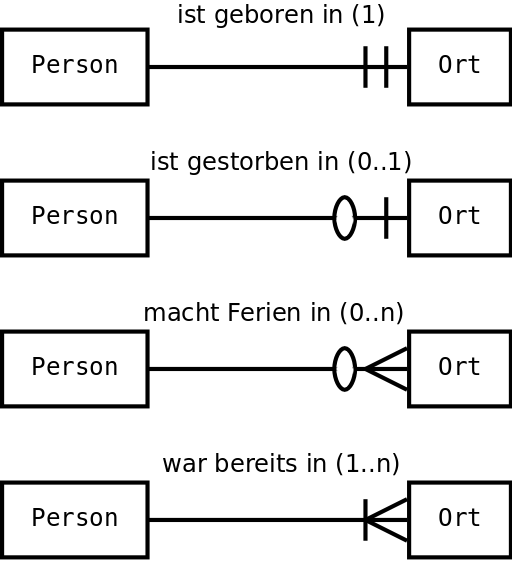
\includegraphics[scale=0.7]
	{Datenbank_Kardinalitaeten.png}
    \caption{Kardinalitäten}
    \label{fig:kardinalitaeten}
\end{figure}
Im ER-Diagramm von Abbildung \ref{fig:erDiagramm} werden Primary-Keys fett und Foreign Keys kursiv dargestellt.

\begin{figure}[H]
	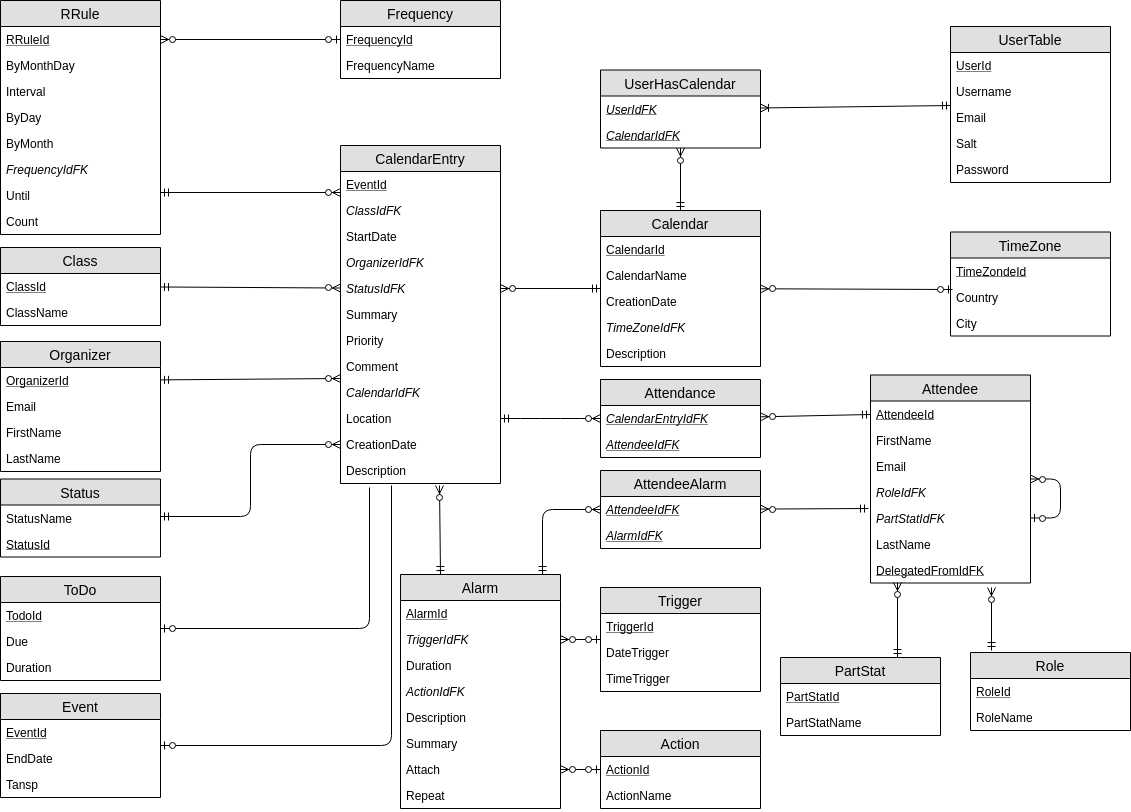
\includegraphics[angle=270,origin=c,width=\textwidth]{Datenbank_ER-Diagramm.png}
    \caption{ER-Diagramm}
    \label{fig:erDiagramm}
\end{figure}

\subsubsection*{Benutzer und Kalender}
\label{ref:benutzerKalender}
In der UserTable-Tabelle werden Benutzerdaten gespeichert. Jeder Benutzer bekommt eine einmalige ID zugewiesen, die UserId. Weiters wird von jedem Benutzer ein Benutzername, eine Email-Adresse und ein Passwort gespeichert. Genaueres zum UserTable ist im Kapitel \ref{sec:UserDB}. Da ein Benutzer mehrere Kalender haben kann und ein Kalender auch zu mehreren Benutzern gehört, gibt es die Tabelle UserHasCalendar, welche dazu dient, festzuhalten welcher Kalender zu welchen Benutzern gehört. Dies wird erreicht indem der Primary-Key der UserTable-Tabelle und der Calender-Tabelle zusammen als Primary-Key in der UserHasCalender-Tabelle genommen werden.Wie dies im ER-Diagramm aussieht ist in Abbildung \ref{fig:userCalender} zu sehen.\\
Die Calender-Tabelle speichert Informationen zu einem Kalender welche dann im Parser in die iCal-Datei gegeben werden.
\begin{figure}[H]
	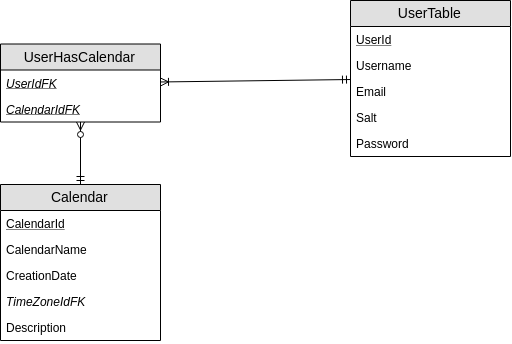
\includegraphics[width=\textwidth]{Datenbank_UserCalendar.png}
    \caption{Relation zwischen Benutzer und Kalender}
    \label{fig:userCalender}
\end{figure}

\subsubsection*{Kalender und Zeitzonen}
\label{ref:kalenderZeitzonen}
Da dieses Projekt für ein Unternehmen gemacht wurde, welches mit Internationalen Kunden tätig ist, ist es wichtig, dass Kalender in verschiedenen Zeitzonen sein können. Deswegen wurde eine eigene Tabelle mit Zeitzonen angefertigt, damit das Hinzufügen von einer Zeitzone in einen Kalender einfacher wird. Die TimeZone-Tabelle welche Zeitzonen abbildet besteht aus einer einmaligen ID, dem Land und der Stadt der Zeitzone, da im iCal-Format Zeitzonen so abgebildet werden.  Wie dies im ER-Diagramm abgebildet ist, ist in Abbildung \ref{fig:timezoneCalender} zu sehen.
\begin{figure}[H]
	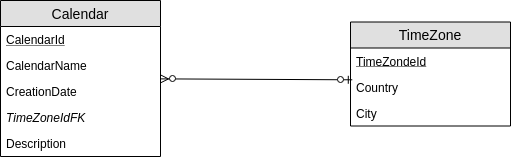
\includegraphics[width=\textwidth]{Datenbank_CalendarTimezone.png}
    \caption{Relation zwischen Kalender und Zeitzone}
    \label{fig:timezoneCalender}
\end{figure}

\subsubsection*{Kalendereinträge}
\label{ref:kalenderEintraege}
Ein Kalender besteht aus mehreren Kalendereinträgen. Ein Kalendereintrag ist zum Beispiel ein Termin oder ein To-Do Element. Termine werden in der Event-Tabelle und To-Dos in der ToDo-Tabelle abgebildet, dies ist in Abbildung \ref{fig:calendarEntries} zu sehen. Da diese beiden Objekte viele ähnliche Attribute haben aber dennoch einige Attribute besitzen welche die andere Tabelle nicht benötigt, sind beide mit der gleichen Supertabelle über eine is-a Relation verbunden. Is-a bedeutet, dass beide Tabellen alle Attribute der CalendarEntry-Tabelle zusätzlich zu ihren eigenen Attributen besitzen.
\begin{figure}[H]
	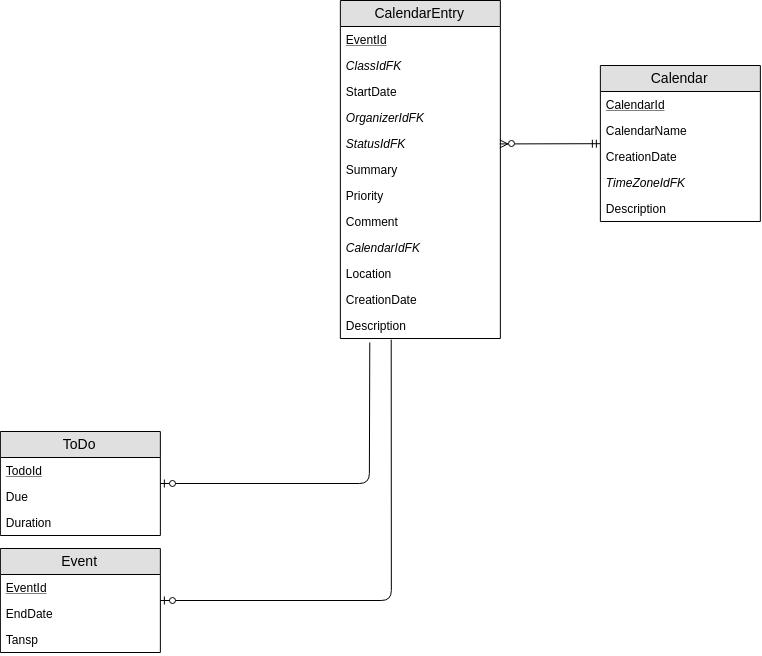
\includegraphics[width=\textwidth]{Datenbank_CalenderEntries.png}
    \caption{Kalendereinträge}
    \label{fig:calendarEntries}
\end{figure}

\subsubsection*{Kalendereintragseigenschaften}
\label{ref:kalendereintragseigenschaften}
Einträge wie VEVENT und VTODO in iCal-Dateien haben eine Vielzahl an Attributen. Diese Attribute werden in der Datenbank durch Eins zu Mehrere Beziehungen abgebildet. Die Attribute welche in der Datenbank mit der CalendarEntry-Tabelle verbunden sind und für alle Einträge in einer iCal-Datei zur Verfügung stehen sind nur mit der CalendarEntry-Tabelle verbunden anstatt mit der ToDo- oder Event-Tabelle. Die Tabellen RRUle, Class, Organizer und Status wurden in eigene Tabellen ausgebaut, da so keine Fehler auftreten können. Zum Beispiel kann so kein Status in einen Kalendereintrag eintragen welcher nicht existiert, denn es gibt nur eine bestimmte Anzahl an vorgefertigten Einträge welche das iCal-Format erlaubt. Deswegen sind die Status- und Class-Tabelle schon von Haus aus gefüllt. Wie dies im ER-Diagramm aussieht ist in Abbildung \ref{fig:kalendereintragseigenschaften} ersichtlich.\\
In der Class-Tabelle gibt es die Einträge: PUBLIC, PRIVATE und CONFIDENTIAL. In der Status Tabelle gibt es für für ToDo- und Event-Einträge verschiedene Einträge. Da in der Datenbank die Status-Tabelle nicht mit einer Event oder einer ToDo-Tabelle verbunden ist macht das in der Datenbank keine Probleme. Ob ein Status eines ToDo-Elements in einem Event verwendet wird wird im Parser abgefragt. Inhalte der Status Tabelle sind: TENTATIVE, CONFIRMED, CANCELLED, NEEDS-ACTION, COMPLETED, IN-PROCESS und CANCELLED. Genaueres zur Funktionsweise dieser Attribute im Kapitel \ref{sec:keywords}.
\begin{figure}[H]
	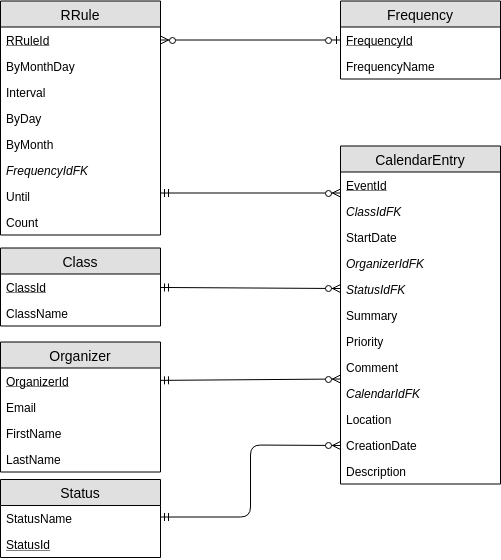
\includegraphics[width=\textwidth]{Datenbank_Attribute.jpg}
    \caption{Kalendereintragseigenschaften}
    \label{fig:kalendereintragseigenschaften}
\end{figure}

\subsubsection*{Teilnehmer}
\label{ref:teilnehmer}
Im iCal-Format können Termine an Teilnehmer zuweisen. Diese Teilnehmer benötigen eine Email-Adresse sowie einen Vor- und Nachnamen. Weiters gibt es für Teilnehmer eine Rolle welche in der Role-Tabelle abgebildet wird und einen Status ob der gefragte Teilnehmer bereits zugesagt hat, dies wird in der PartStat-Tabelle abgebildet. Rollen könnten sein: CHAIR, REQ-PARTICIPANT, OPT-PARTICIPANT und NON-PARTICIPANT, für den Zustand der Annahme gibt es unterschiedliche Zustände für Events und Todos, jedoch sind beide in der selben Tabelle abgebildet: NEEDS-ACTION, ACCEPTED, DECLINED, TENTATIVE, DELEGATED, COMPLETED und IN-PROCESS.\\
Da ein Kalendereintrag mehrere Teilnehmer haben kann, wird die Tabelle Attendance benötigt, welche verwaltet welche Teilnehmer in welchen Kalendereinträgen stehen sollen. Wie die Abbildung der Teilnehmer im ER-Diagramm modelliert wurde, ist in Abbildung \ref{fig:datenbankTeilnehmer} ersichtlich.\\
Ein Alarm kann, wenn er auslöst, eine Email-Benachrichtigung aussenden. Diese Email wird dann an alle Teilnehmer versendet, welche im Alarm festgelegt worden sind. Da ein Alarm mehrere Teilnehmer haben kann und ein Teilnehmer wiederum mehrere Alarme haben kann, wird die Tabelle AttendeeAlarm benötigt um festzustellen welcher Teilnehmer zu welchen Alarmen gehört.
\begin{figure}[H]
	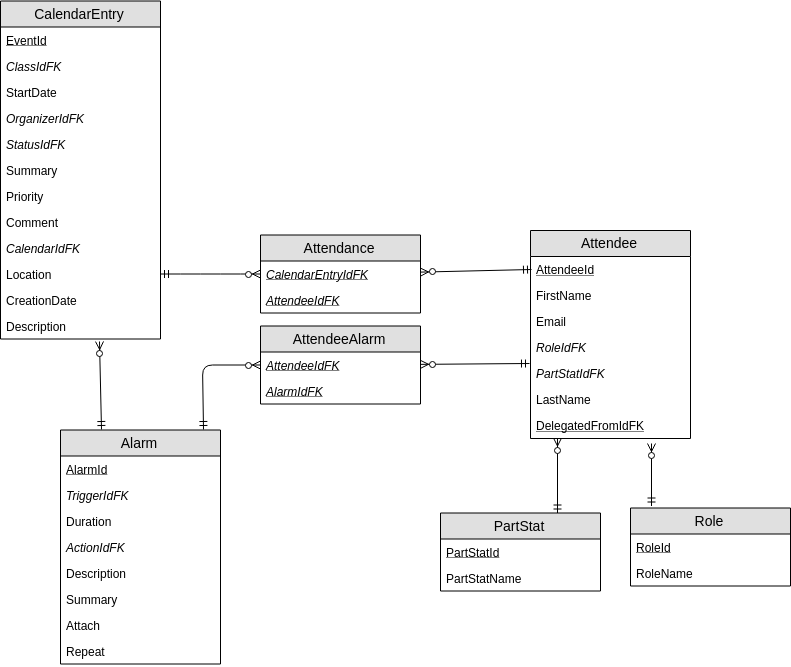
\includegraphics[width=\textwidth]{Datenbank_Attendee.png}
    \caption{Teilnehmer}
    \label{fig:datenbankTeilnehmer}
\end{figure}
\pagebreak